\documentclass[a4paper,12pt,fleqn]{article}
\usepackage[utf8]{inputenc}
%
\usepackage[T1]{fontenc}
\usepackage{lmodern}
%
\usepackage{ngerman}
\usepackage{amsmath}
\usepackage{amssymb}
\usepackage{color}
\definecolor{c1}{RGB}{00,40,80}
\usepackage[colorlinks=true,linkcolor=c1]{hyperref}
%\usepackage{geometry}
%\geometry{a4paper,left=25mm,right=15mm,top=20mm,bottom=28mm}
\usepackage{graphicx}
\begin{document}

\begin{center}
\begin{LARGE}
\noindent
\textbf{Die Ableitung bei beliebigen\\
Objekten}
\end{LARGE}
\\
\vspace{2mm}
\begin{large}
Feb. 2016
\end{large}
\end{center}

\tableofcontents
\vspace{4mm}
\noindent
\textbf{Zusammenfassung}. In diesem Artikel soll es darum gehen,
wie das Konzept der Ableitung von der Vorstellung einer reellen
Funktion befreit werden kann. Bei der Ableitung geht es um das
Problem, wie eine Tangente an den Graph der Funktion gelegt wird.
Dieses Prinzip soll auf beliebige {\glqq}smoothe{\grqq} Objekte
übertragen werden.

\newpage
\section{Kurven}
\subsection{Ableitung einer Funktion}

Von einer Funktion \(f{:}\;I{\rightarrow}\mathbb R\) mit einem
offenen Intervall \(I{\subseteq}\mathbb R\) lässt sich an einer
Stelle \(x_0{\in}I\) die Ableitung berechnen. Diese ist definiert
durch
\begin{equation}
(Df)(x_0) := \lim_{h\rightarrow 0} \frac{f(x_0+h)-f(x_0)}{h}.
\end{equation}
Die Funktion \(f\) wird an der Stelle \(x_0\) differenzierbar genannt,
wenn dieser Grenzwert existiert, d.h. wenn rechtsseitiger und
linksseitiger Grenzwert endlich sind und übereinstimmmen.

Die Ableitung gibt den Anstieg der Tangente an, welche den Graph
der Funktion \(f\) am Punkt \((x_0,f(x_0))\) berührt. Diese
Tangente kann also durch die affine Funktion
\begin{equation}
T(x) = f(x_0)+(Df)(x_0)(x-x_0)
\end{equation}
dargestellt werden.

Hier macht man nun zwei Beobachtungen. Erstens sieht der Graph einer
differenzierbaren Funktion \(f\) an der Stelle \(x_0\) unter einer
stark vergrößernden Lupe so aus wie der Graph der Tangentenfunktion
\(T\). D.h. \(f\) lässt in einer hinreichend kleinen
Umgebung \(U(x_0)\) hinreichend gut durch \(T\) approximieren.

Zweitens: Um die Tangente zu bestimmen ist nur der Graph von \(f\)
entscheidend. Daher kann man sich auch eine Kurve im \(\mathbb R^2\)
denken, die genau den Graph von \(f\) wiedergibt. Was wir nun tun
wollen ist klar. Wir müssen uns von der Vorstellung einer reellen
Funktion befreien und stattdessen das Konzept einer Kurve als
geometrisches Objekt möglichst klar herausstellen. Denn nur die
Kurve selbst ist bei der Bestimmung der Tangente entscheidend.

\subsection{Darstellung einer Kurve}

Eine Kurve \(c\) ist eine mit einem Stift gezogene Linie auf einem
unendlich großen weißen Blatt Papier. Zu dieser Vorstellung wollen
wir uns voranarbeiten.

Zunächst denken wir uns das große Blatt Papier als euklidische
Ebene. In dieser Ebene kann ein Punkt \(P\) als Ursprungspunkt
gewählt werden, womit die Ebene zu einem Vektorraum wird.
Jetzt wählt man noch eine Orthonormalbasis \(B=(e_1,e_2)\).
Hierdurch wird ein Koordinatensystem \((P,B)\) festgelegt.

Wir denken uns nun eine Funktion \(r{:}\; I{\rightarrow}\mathbb R^2\).
Das Argument von \(r\) soll als Parameter \(t\) bezeichnet werden,
der Wert \(r(t)\) ist ein Tupel \((x,y)\). Die Werte dieser Funktion
sollen nun genau im Koordinatensystem \((P,B)\) liegen. Der
Funktionswert ist also von der Gestalt
\begin{equation}
r(t) = \begin{bmatrix}
x(t)\\ y(t)
\end{bmatrix}
= P+x(t)e_1+y(t)e_2.
\end{equation}
Diese Gleichung ist nur als Entsprechung zu verstehen. Die linke Seite
ist ein Koordinatentupel (Koordinatenvektor), also ein Punkt im
Koordinatenraum \(\mathbb R^2\). Die rechte Seite
ist ein Punkt der euklidischen Ebene \(E_2\).

Jetzt ist die Bildmenge \(\mathrm{Bild}(r)\) eine solche
Kurve \(c\). Damit ist unser Ziel erreicht. Nun gibt es Kurven
aber auch im Raum und in höherdimensionalen Räumen. Für solche
Kurven im euklidischen Punktraum \(E_n\) gilt dann einfach
\begin{equation}
r(t) = p+x_1(t)e_1+\ldots+x_n(t)e_n.
\end{equation}

\subsection{Ableitung einer Kurve}

Wie bestimmt man nun zu einer gegebenen Kurve \(c=\mathrm{Bild}(r)\)
an einem Punkt \(r(t_0)\in c\) die Tangente? Nun, zunächst kann man
\(r(t)\) ja einfach nach \(t\) ableiten. Der Ableitungsoperator
ist ein linearer Operator. Konstante Vektoren behandelt man einfach
wie konstante Zahlen. Damit ergibt sich
\begin{gather*}
r'(t) = Dr(t) = D(P+x(t)e_1+y(t)e_2)\\
= DP+Dx(t)e_1+Dy(t)e_2 = x'(t)e_1+y'(t)e_2.
\end{gather*}
Man stellt fest, dass die Information über den Ursprungspunkt \(P\)
beim Ableiten verloren geht. Das Objekt \(r'(t_0)\) ist also ein
Vektor im Vektorraum \(\mathrm{span}(B)\) mit \(B=(e_1,e_2)\).

Es ist nun so, dass dieser Vektor \(r'(t_0)\) ein Tangentialvektor
von \(c\) am Punkt \(r(t_0)\) ist. Wie können wir das rechtfertigen?
Nun, dazu betrachtet man den Verbindungsvektor von \(r(t)\) nach
\(r(t+h)\). Anmerkung: dieser Verbindungsvektor ist genau das selbe
wie der Verschiebungsvektor von \(r(t)\) nach \(r(t+h)\).
Und nun lässt man \(h\) gegen null laufen, sodass dieser
Verbindungsvektor immer ähnlicher zu einem Tangentialvektor an dieser
Stelle wird. Wie lang ein Tangentialvektor ist, ist unbedeutend.
Wichtig ist nur die Richtung.

Leider wird der Verbindungsvektor \(r(t+h)-r(t)\) immer kürzer
und verschwindet, wenn \(h\) gegen null geht. Das ist dumm. Um dieses
Problem zu beheben, machen wir den Verbindungsvektor künstlich länger,
indem wir durch die kleine Zahl \(h\) teilen bzw. mit der großen
Zahl \(1/h\) multiplizieren. Man rechnet nun
\begin{gather*}
\frac{r(t+h)-r(t)}{h}
= \frac{P+x(t+h)e_1+y(t+h)e_2-P-x(t)e_1-y(t)e_2}{h}\\
= \frac{x(t+h)-x(t)}{h}e_1 + \frac{y(t+h)-y(t)}{h}e_2.
\end{gather*}
Im Grenzfall (\(h\) gegen null) gilt also
\[r'(t) = x'(t)e_1+y'(t)e_2\]
womit \(r'(t)\) tatsächlich ein Tangentialvektor an der Stelle \(t\)
ist.

Dieser Vektor \(r'(t)\) kann auch als Geschwindigkeitsvektor \(v(t)\)
interpretiert werden, seine Länge ist die Momentangeschwindigkeit,
wenn \(t\) als Zeit und \(r(t)\) als Ort interpretiert wird.
Das soll uns hier aber nicht weiter interessieren.
Um besser klarzustellen, dass die Länge von \(v(t)\)
nicht von Bedeutung ist, kann man diesen auch normieren.
D.h. man teilt durch seine eigene Länge \(|v(t)|\).
Man erhält den Einheitstangentialvektor
\begin{equation}
\hat v(t) := \frac{v(t)}{|v(t)|} = \frac{r'(t)}{|r'(t)|}.
\end{equation}
Nun gilt \(|\hat v(t)|=1\) für alle Parameterwerte \(t\).

Die Tangente ist nun gegeben durch die Parameterdarstellung
\begin{equation}
T(t) = r(t_0)+\hat v(t_0)(t-t_0).
\end{equation}
Die Tangente ist dann einfach die Bildmenge \(\mathrm{Bild}(T)\).
Diese Bildmenge ist ein affiner Unterraum der euklidischen
Ebene. Wählt man \(r(t_0)\) als Ursprungspunkt, so wird dieser Raum
zu einem Vektorraum, dem sogenannten \textit{Tangentialraum} der
Kurve \(c\) am Anschmiegepunkt \(r(t_0)\in c\). Dieser
eindimensionale Tangentialraum ist einfach der durch den
einen Basisvektor \(r'(t_0)\) aufgespannte Vektorraum.

Anschaulich klar ist nun, dass der Tangentialraum am Punkt \(r(t_0)\)
nur von der Kurve \(c\) abhängig ist, aber nicht von der gewählten
Parameterdarstellung. Wie überprüft man das?

Dazu betrachten wir eine sogenannte \textit{Umparameterisierung}
\(\varphi\). Bei \(\varphi\) soll es sich um eine bijektive
reelle Funktion handeln, welche \(t_0\) als Fixpunkt hat und
differenzierbar ist. Die Fixpunkteigenschaft bedeutet einfach
\(\varphi(t_0)=t_0\). Jetzt ist
\begin{equation}
r_2(t) = (r\circ\varphi)(t):=r(\varphi(t))
\end{equation}
eine neue Parameterdarstellung der selben Kurve \(c\).
Wir müssen nun zeigen, dass sich der Einheitstangentialvektor
nicht ändert. Dabei wird erst die Kettenregel und dann die
Fixpunkteigenschaft verwendet. Es ergibt sich
\begin{gather*}
\frac{r_2'(t_0)}{|r_2'(t_0)|}
= \frac{(r\circ\varphi)'(t_0)}{|(r\circ\varphi)'(t_0)|}
= \frac{(r'\circ\varphi)(t_0)\varphi'(t_0)}{|(r'\circ\varphi)(t_0)||\varphi'(t_0)|}
= \frac{r'(t_0)}{|r'(t_0)|} \mathrm{sgn}(\varphi'(t_0)).
\end{gather*}
Bis auf das Vorzeichen stimmen beide Einheitstangentialvektoren
überein. Damit ergibt sich der gleiche Tantentialraum. Wenn die
Umparameterisierung orientierungserhaltend ist, wenn also
\(\mathrm{sgn}(\varphi'(t))=1\) für alle \(t\) ist, so stimmen
beide Einheitstangentialvektoren völlig überein.

Anmerkung: Auf einem offenen Intervall definierte bijektive
stetige reelle
Funktionen sind entweder überall streng monoton steigend oder überall
streng monoton fallend. Differenzierbare Funktionen sind auch stetig.
Somit handelt es sich bei \(\mathrm{sgn}(\varphi'(t))\) um eine
Konstante, die nicht von \(t\) abhängig ist.

\section{Flächen}
\subsection{Parameterflächen}
Nach unserem gegenwärtigen Verständnis ist die Ableitung so etwas
wie die Information über den Tangentialraum einer Kurve \(c\) an
einem bestimmten Punkt auf dieser Kurve. Diese Idee wollen wir nun
auf krumme Flächen übertragen. Man kann sich ja vorstellen, dass
eine Kugeloberfläche (Sphäre) eine Tangentialebene an einem bestimmten
Punkt \(p\) auf dieser Kugeloberfläche hat. Anschaulich gesprochen:
Wir lehnen ein Buch an einen Ball.

Es bietet sich an, ein bestimmtes Objekt als Beispiel zu verwenden,
an dem Ideen und Formalismen ausgetestet werden können.
Eine Kugeloberfläche ist ein recht hässliches Objekt. Ich will etwas
einfacheres als Studienobjekt verwenden: die Oberfläche eines Torus.

Man kann sich nun eine solche Fläche vorstellen, die in den
euklidischen Punktraum eingebettet ist. Für eine Parameterdarstellung
braucht man jetzt zwei Parameter \(u,v\). Ist \(P\) ein Punkt
des euklidischen Punktraumes und \(B=(e_1,e_2,e_3)\) eine
Orthonormalbasis, so kann man die Parameterdarstellung
\begin{equation}\label{Flaeche}
r(u,v) = P+x(u,v)e_1+y(u,v)e_2+z(u,v)e_3.
\end{equation}
benutzen. Durch die Verwendung dieses Koordinatensystems \((P,B)\)
können wir uns \(r(u,v)\) auch wieder als Tupel im Koordinatenraum
denken. Also als
\begin{equation}
r(u,v) = (x(u,v),y(u,v),z(u,v)).
\end{equation}
Eine solche Darstellung wollen wir nun für die Torusoberfläche
angeben. Der Mittelkreis soll den Radius \(R\) haben, die Tube
den Radius \(r\). Wie konstruiert man das?

Der Mittelkreis ist ja durch die Koordinaten \((R\cos u,R\sin u,0)\)
parameterisiert, wobei \(0\le u<2\pi\) ist. Wir brauchen nun
einen zweiten Vektor, der hinzuaddiert wird. Dieser hat für \(v=0\)
die selbe Richtung wie der Mittelkreisvektor und dreht sich dann um
den Querschnitt der Tube. Und jetzt? Mit Kugelkoordinaten kann man
so etwas darstellen. Die will ich jetzt nicht herleiten. Man hat
dann einfach den Vektor
\begin{equation}
\begin{bmatrix}
x\\ y\\ z
\end{bmatrix}
= \begin{bmatrix}
r\cos u\sin v\\
r\sin u\sin v\\
r\cos v
\end{bmatrix}.
\end{equation}
Hierbei ist \(u\) die Länge und \(v\) die Breite. Für \(v\) wählt man
am besten \(0\le v<2\pi\). Die beiden Koordinatenvektoren addiert man
und erhält
\begin{equation}\label{Torus}
\begin{bmatrix}
x\\ y\\ z
\end{bmatrix}
= \begin{bmatrix}
R\cos u\\
R\sin u\\
0
\end{bmatrix}+\begin{bmatrix}
r\cos u\sin v\\
r\sin u\sin v\\
r\cos v
\end{bmatrix}
= \begin{bmatrix}
(R+r\sin v)\cos u\\
(R+r\sin v)\sin u\\
r\cos v
\end{bmatrix}.
\end{equation}

\subsection{Die Richtungsableitung}
Bevor wir versuchen Tangentialebenen an den Torus zu legen, kümmern
wir uns um eine wesentliche Verallgemeinerung der Ableitung. Dazu
denken wir uns eine Funktion \(f\) mit Definitionsbereich
\(D(f)\subseteq\mathbb R^2\) und Zielmenge \(Z(f)=\mathbb R\).
Man kann sich vorstellen, dass \(f\) jedem Punkt \((x,y)\) der
Koordinatenebene eine Höhe \(f(x,y)\) zuordnet. Nun soll \(v\) ein
Verschiebungsvektor in der Koordinatenebene sein. Hierdurch
wird am Punkt \(r_0=(x_0,y_0)\) eine Gerade und senkrecht zur
Koordinatenebene eine Ebene festgelegt. Entlang dieser
Geraden gibt es auf der senkrechten Ebene eine Schnittkurve.
Die Gerade in der Koordinatenebene ist gegeben durch
den affinen Unterraum
\begin{equation}
g = r_0+\mathrm{span}(v).
\end{equation}
Eine Parameterdarstellung für die Gerade ist
\begin{equation}
g(t) = r_0+tv.
\end{equation}
Anschaulich gesprochen skaliert die reelle Zahl \(t\) den
Verschiebungsvektor \(v\), sodass man zu allen Punkten auf der
Geraden gelangt, wenn \(t\) variiert wird.
Der affine Unterraum ist dann \(\mathrm{Bild}(g)\).

Die Schnittkurve ist dann die Bildmenge der Einschränkung
(Restriktion) von \(f\) auf \(g\cap D(f)\). Die Einschränkung
ist eine reelle Funktion, und von so einer lässt sich die
gewöhnliche Ableitung bestimmen. Diese Restriktion wollen wir
als \(f_r\) bezeichnen. Dabei ergibt sich
\(f_r(t) = f(r_0+tv)\).
Die Ableitung ist
\begin{equation}\label{Restriktion}
f_r'(t) = \frac{\mathrm d}{\mathrm dt} f(r_0+tv).
\end{equation}
Den Tangentenanstieg \(f_r'(0)\) wollen wir als Richtungsableitung
bezeichnen. Die Richtungsableitungen in Richtungen, welche
parallel zu den Koordinatenachsen \((x,0)\) und \((0,y)\) sind,
bezeichnen wir als partielle Ableitungen. Genauer gesagt muss man
hierbei einen normierten Vektor verwenden. D.h. es soll \(|v|=1\) sein.
Für die Richtungsableitung in Richtung \(v\) schreibt man \(D_v\) oder
\(D[v]\). Für die partiellen Ableitungen dementsprechend
\(D_x\) und \(D_y\).

Für \(D_x\) nimmt man nun den normierten Vektor \(v=(1,0)\).
Damit ergibt sich
\begin{gather*}
(D_x f)(x_0,y_0) = f_r'(0)
= \frac{\mathrm d}{\mathrm dt} f(x_0+1t,y_0+0t)\Big|_{t=0}\\
= \lim_{h\rightarrow 0} \frac{f(x_0+t+h,y_0)-f(x_0+t,y_0)}{h}\Big|_{t=0}\\
= \lim_{h\rightarrow 0} \frac{f(x_0+h,y_0)-f(x_0,y_0)}{h}.
\end{gather*}
Eine partielle Ableitung berechnet man also einfach, indem man
die Variable, nach der nicht abgeleitet wird, als Konstante
betrachtet und dann normal ableitet. In diesem Fall setzt man einfach
\(y\) konstant. Damit kann mit partiellen Ableitungen rechnen,
als würde man mit gewöhnlichen Ableitungen rechnen. Wählt man
stattdessen \(v=(1,2)\), so kann man auf diese Art nicht mehr
rechnen.

Es gibt aber auch einen Formalismus, um Richtungsableitungen
in beliebige Richtungen praktisch bestimmen zu können.
Zunächst fasst man alle Ableitungen zum formalen Vektor
\begin{equation}
\nabla = D_x e_1+D_y e_2
\end{equation}
zusammen, welcher als Nabla-Vektor bezeichnet wird. Nun ist das
Standardskalarprodukt zweier Koordinatenvektoren \((v,w)\) definiert
durch
\begin{equation}
\langle v,w\rangle := \sum_k v_k w_k = v_1 w_1+v_2 w_2.
\end{equation}
Speziell für die Orthonormalbasis gilt daher
\begin{equation}
\langle e_i,e_j\rangle = [i=j].
\end{equation}
Es ist \([A]=0\) falls die Aussage \(A\) falsch ist, und \([A]=1\)
falls \(A\) wahr ist. Die Skalarprodukte von anderen Basen können
berechnet werden, indem die Basisvektoren als Linearkombination
von Orthonormalbasen dargestellt werden.

Nun gilt für die Formel (\ref{Restriktion}) die Kettenregel
in der Gestalt
\begin{equation}
f_r'(t) = \langle\frac{\mathrm d}{\mathrm dt}(r_0+tv),
(\nabla f)(r_0+tv)\rangle
= \langle v,(\nabla f)(r_0+tv)\rangle.
\end{equation}
Wir rechnen also innere mal äußere Ableitung, nur dass das
\textit{mal} in diesem Fall das Skalarprodukt ist. Hiermit ergibt
sich
\begin{equation}
(D_v f)(r_0) = f_r'(0) = \langle v,(\nabla f)(r_0)\rangle.
\end{equation}
Da das Skalarprodukt bilinear ist kann man \(f\), als Skalar
betrachtet, formal aus dem Skalarprodukt herausziehen.
Als Merkformel ergibt sich die funktionale Gleichung
\begin{equation}\label{Richtungsableitung}
D_v = \langle v,\nabla\rangle = v_1D_1+v_2D_2.
\end{equation}
Meiner Meinung nach doch ein ganz ästhetisches Resultat.
Ausgeschrieben lautet die Formel
\begin{equation}\label{RAexpandiert}
(D_v f)(r_0) = v_1(D_1 f)(r_0)+ v_2(D_2 f)(r_0).
\end{equation}
Damit haben wir die Berechnung der Richtungsableitung auf
die Berechnung der partiellen Ableitungen zurückgeführt.

Schließlich lassen sich die hier dargestellten Schlussfolgerungen
in direkter Weise auf Funktionen von beliebig vielen Variablen
verallgemeinern. Eine solche Funktion wollen wir auch als Skalarfeld
auf dem Koordinatenraum bezeichnen, denn jedem Punkt des
Koordinatenraumes wird durch die Funktion ein Skalar zugeordnet.

\subsection{Skalarfelder}
Sei \(r=(x,y)\). Die Bildmenge des Skalarfeldes \(f(r)\) lässt sich
nun als Oberfläche betrachten. Damit hat das Skalarfeld am
Punkt \((r,f(r))\) eine Tangentialebene. Wie stellt man diese
nun dar? 

Eine Ebene lässt sich allgemein Darstellen durch
eine affine Funktion in zwei Variablen, also eine Funktion der
Form
\[T(x,y) = z_0 + m_x (x-x_0)+ m_y (y-y_0).\]
Bei der Tangentialebene stimmen die Anstiege \(m_x\) und \(m_y\)
nun aber mit den partiellen Ableitungen \(D_x f(r_0)\) und \(D_y f(r_0)\)
überein. Außerdem gilt \(z_0=f(r_0)\). Somit ergibt sich
\begin{equation}
T(x,y) = f(r_0)+D_xf(r_0)(x-x_0)+D_y f(r_0)(y-y_0).
\end{equation}
In Kurzform lautet die Formel
\begin{equation}
T(r) = f(r_0)+\langle (\nabla f)(r_0),r-r_0\rangle.
\end{equation}
In dieser Form gilt die Formel für Skalarfelder von beliebig
vielen Variablen. Unsere wesentliche Beobachtung ist, dass
\(\nabla\) ein Operator ist, der einem Skalarfeld an jeder Stelle
\(r_0\) die Information über den Tantentialraum dort zuordnet.
Man kann als von einer verallgemeinerten Ableitung sprechen. Für
reelle Funktionen (als Skalarfeld von einer einzigen Variablen)
ergibt sich hieraus wieder die gewöhnliche Ableitung.
Damit haben wir ein Etappenziel erreicht.

\subsection{Tangentialräume}

Allgemeiner als bei einem Skalarfeld soll eine Oberfläche nun
durch eine Parameterdarstellung gegeben sein. Ein Skalarfeld kann
nämlich als spezielle Parameterdarstellung angesehen werden.
Wenn also \(f(x,y)\) ein Skalarfeld ist, so setzt man
\begin{gather*}
x:=u,\qquad y:=v,\qquad z:=f(u,v).
\end{gather*}
Damit ergibt sich die spezielle Parameterdarstellung
\begin{equation}
r(u,v) = ue_1+ve_2+f(u,v)e_3.
\end{equation}
Eine Fläche lässt nun aber selbst als eine gekrümmte euklidische
Ebene ansehen. Unter einer stark vergrößernden Lupe kann die
Fläche gut durch eine Ebene approximiert werden, eben durch die
Tangentialebene dort.

So wie man in der euklidischen Ebene ein Koordinatensystem
festlegen kann, kann man auf der gekrümmten Fläche auch
ein Koordinatensystem festlegen. Oft ist es aber nicht möglich
ein globales Koordinatensystem festzulegen.

Nun ist es so, dass durch die Parameter \(u,v\) schon ein
gekrümmtes Koordinatensystem auf der Oberfläche festgelegt wird.
Die Koordinatenlinien erhält man, indem man jeweils \(u\) oder \(v\)
konstant hält. Bei den partiellen Ableitungen
\begin{equation}
(D_u r)(u_0,v_0),\quad (D_v r)(u_0,v_0)
\end{equation}
handelt es sich um Tangentialvektoren am Punkt \((u_0,v_0)\).
Wenn diese nicht kollinear sind, so spannen sie den
Tangentialraum dort auf. Fast man beide partiellen Ableitungen
nebeneinander zusammen, so erhält man die Jacobi-Matrix
\begin{equation}
J[r] = \begin{bmatrix}
D_u r_x & D_v r_x\\
D_u r_y & D_v r_y\\
D_u r_z & D_v r_z
\end{bmatrix}.
\end{equation}
Fast man die beiden partiellen Ableitungen nebeneinander
zusammen, so ergibt sich
\begin{equation}
\nabla\otimes r = \begin{bmatrix}
D_u r_x & D_u r_y & D_u r_z\\
D_v r_x & D_v r_y & D_v r_z
\end{bmatrix}.
\end{equation}
Damit gilt \(J[r]=(\nabla\otimes r)^T\). Bei \(\nabla\otimes r\)
handelt es sich also um eine natürliche Verallgemeinerung
des Gradienten auf eine vektorwertige Funktion. Man spricht
daher auch vom Vektorgradient. Falls die vektorwertige Funktion
nur eine einzige Komponente hat, ergibt sich als Spezialfall
wieder der gewöhnliche Gradient.

Für gekrümmte Koordinatensystem gibt die Jacobimatrix bzw. der
Vektorgradient also nun die Information über den Tangentialraum
an. Dabei ist es eigentlich auch egal, ob das Koordinatensystem nun
auf eine gekrümmte Fläche aufgebügelt ist, oder nicht. Man kann
auch bei ebenen gekrümmten Koordinatensystemen von Tangentialräumen
sprechen.

Wie müssen hier zwischen äußerer und innerer Krümmung unterscheiden.
Äußere Krümmung bedeutet, dass ein ebenes Blatt Papier gebogen
wird. Innere Krümmung bedeutet, dass das Koordinatensystem auf
dem ebenen Blatt Papier verzerrt wird, ohne das Blatt zu verbiegen.
In beiden Fällen entarten die Vektorräume, welche an jeden Punkt
der euklidischen Ebene angeheftet sind, zu Tangentialräumen.

Um es abstrakter auszudrücken: Tangentialräume sind lineare
Approximationen von nichtlinearen Objekten. Genau das macht
die Ableitung. Sie ordnet einem nichtlinearen Objekt an jedem
Punkt \(p\) dieses Objektes die Information über die lineare
Approximation dort zu.

\subsection{Skalarfelder auf krummen Flächen}

Wir gehen jetzt noch einen Schritt weiter.
Auf einer krummen Fläche lässt sich doch auch ein
Skalarfeld definieren. Jedem Koordinatenpunkt \((u_1,u_2)\)
des krummlinigen Koordinatensystems lässt sich doch
ein Funktionswert \(f(u_1,u_2)\) zuordnen. Man denke sich zum Beispiel
die Temperaturverteilung auf einer Torusoberfläche die von einer
bestimmten Richtung aus von der Sonne beschienen wird. Jedem Punkt
auf der Torusoberfläche lässt sich eine Temperatur zuordnen.
Das ist ein typisches Beispiel für ein Skalarfeld.

Wie bestimmt man nun die Richtungsableitung? Herbei muss man sich
bewusst sein, dass es durch die krumme Form des Raumes nicht mehr
einfach einen Verschiebungsvektor geben kann, weil es solche nur für
ungekrümmte affine Räume gibt.

Die Idee ist nun eine Parameterkurve \(\gamma(t)\) zu definieren die den
Tangentialvektor \(v=\gamma'(0)\) hat. Diese Kurve soll auf der
krummen Oberfläche verlaufen. Sei \(r=(u_1,u_2)\). Nun ist
\(r_0=\gamma(0)\). Als lineare Approximation von \(\gamma\) ergibt
sich die Parametergerade
\begin{equation}
g(t) = \gamma(0)+t\gamma'(0) = r_0+tv.
\end{equation}
Damit sieht die Parametergerade \(g\) unter einer stark vergrößernden
Lupe fast genauso aus wie die Parameterkurve \(\gamma\). Daher
ist es legitim, \(g\) in einer kleinen Umgebung durch \(\gamma\)
auszutauschen. Wir erinnern uns nun an Formel (\ref{Restriktion}).
Tauscht man dort aus, so gelangt man zu
\begin{equation}\label{via-gamma}
(D_v f)(r_0) = \frac{\mathrm d}{\mathrm dt}f(\gamma(t))\Big|_{t=0}
= (f\circ\gamma)'(0).
\end{equation}
Mit dieser Formel lassen sich Richtungsableitungen auch
in krummlinigen Koordinatensystemen berechnen.

Man muss sich hier überlegen, dass es zunächst keine andere Möglichkeit
der Berechnung gibt. Man könnte am Punkt \(r_0\) einfach erst einmal
den Tangentialraum betrachten. In diesem Tangentialraum liegt auch
\(v\). Aber: Die Funktion \(f\) ist ja außer bei \(r_0\)
gar nicht auf dem Tangentialraum definiert. Daher kann der Ausdruck
\(f(r_0+tv)\) keinen Sinn ergeben, sodass man stattdessen
\(f(\gamma)\) verwenden muss.

Wir würden nun auch gerne für (\ref{via-gamma}) eine Formel
wie (\ref{Richtungsableitung}) haben. Dazu überlegt man sich wieder,
dass die Kettenregel in der Rechnung
\begin{equation}
(f\circ\gamma)'(0)
= \langle \gamma'(t),(\nabla f\circ\gamma)(t)\rangle\Big|_{t=0}
= \langle v,(\nabla f)(r_0)\rangle.
\end{equation}
weiterhin gültig sein soll. Diese Gleichung gilt aber nur,
wenn wir \((\nabla f)(r_0)\) auf eine uns noch unbekannte Art
bilden.

Zunächst benötigen wir den Formalismus mit dem metrischen Tensor.
Dieser tut sich auf, wenn man Basen betrachtet, die nicht
orthonormal sind.

\subsection{Metrischer Tensor}

Wenn man eine nicht orthonormale Basis \(B=(e_1,e_2)\) verwendet,
so kann man das Standardskalarprodukt nicht mehr auf naive Art
auswerten. Da es bilinear ist, kann man es aber ausmultiplizieren.
Beim ausmultiplizieren von artihmetischen Ausdrücken erhält man
\begin{gather*}
(a_1+a_2)(b_1+b_2)
= a_1b_1+a_1b_2+a_2b_1+a_2b_2.
\end{gather*}
Dementsprechend ergibt sich beim Skalarprodukt
\begin{gather*}
\langle a_1e_1+a_2e_2, b_1e_1+b_2e_2\rangle\\
= a_1b_1\langle e_1,e_1\rangle
+ a_1b_2\langle e_1,e_2\rangle
+ a_2b_1\langle e_2,e_1\rangle
+ a_2b_2\langle e_2,e_2\rangle.
\end{gather*}
Wir definieren nun den metrischen Tensor durch
\begin{equation}
g_{ij} := \langle e_i,e_j\rangle.
\end{equation}
Anmerkung: Der metrische Tensor ist symmetrisch, weil das
Skalarprodukt symmetrisch ist. Somit ergibt sich
\begin{equation}\label{SP}
\langle a,b\rangle =  \sum_{ij} a_ib_j g_{ij}.
\end{equation}
Zu jeder Basis gibt es nun eine Dualbasis. Zu jedem Basisvektor
\(e_k\) gibt es einen Basisvektor \(e^k\) der Dualbasis, welcher
zu allen bis auf \(e_k\) ist und dessen Länge der Kehrwert
von \(e_k\) ist. Somit hat man
\begin{equation}\label{dual}
\langle e_k,e^k\rangle = [i=j].
\end{equation}
Jeder Vektor kann nun als Linearkombinationen aus Basisvektoren
der Basis oder aber der Dualbasis dargestellt werden. Die Indizes
von Komponenten bezüglich der Basis sollen ab jetzt oben stehen,
die Indizes von Komponenten bezüglich der Dualbasis unten. Somit
schreibt man
\begin{equation}
a = \sum_k a^k e_k = \sum_k a_k e^k.
\end{equation}
Bei einer Orthonormalbasis fallen Basis und Dualbasis zusammen.

Der Formalismus mit metrischen Tensor ist nun außerordentlich
einfach. Er besteht nur aus zwei Rechenregeln. Erstens: mit dem
metrischen Tensor der Basis lassen sich Indizes senken, mit dem
der Dualbasis heben. Zweitens: Man darf einen Tensor nur über zwei
Indizes kontrahieren, wenn einer davon oben und einer davon unten
steht.

Für die Berechnung des Skalarproduktes ergibt sich hier also
speziell
\begin{equation}
\langle a,b\rangle = \sum_k a^k b_k
= \sum_k \sum_j g_{kj} a^k b^j.
\end{equation}
Hiermit ergibt sich das gleiche Ergebnis wie bei (\ref{SP}).

Auf dem Torus haben wir nun ein krummliniges Koordinatensystem.
Es gibt auch Koordinatensysteme wo die Koordinatenlinien sich
nicht rechtwinklig schneiden. Zu jedem Punkt \(p\) auf der gekrümmten
Fläche gibt es Tangentialvektoren, die dort den Tangentialraum
aufspannen, wenn sie nicht gerade linear abhängig sind.

Daher können wir die Tangentialvektoren als Basisvektoren benutzen.
Ist die Fläche in der Form (\ref{Flaeche}) dargestellt, so sind
die partiellen Ableitungen \((D_u r)(p)\) und \((D_v r)(p)\) die
beiden Tangentialvektoren am Punkt \(p\). Dann ist der metrische Tensor
\begin{equation}
(g_{ij}) = \begin{bmatrix}
\langle D_u r,D_u r\rangle & \langle D_u r, D_v r\rangle\\
\langle D_v r,D_u r\rangle & \langle D_v r, D_v r\rangle
\end{bmatrix}.
\end{equation}
Genauer gesagt handelt es sich hierbei um ein Tensorfeld. Jedem
Punkt \(p=(u_0,v_0)\) auf der Fläche wird ein metrischer Tensor
\begin{equation}
g(p) = g(u_0,v_0) = (g_{ij})(u_0,v_0)
\end{equation}
zugeordnet.

Wir wollen den metrischen Tensor für die Parameterdarstellung
(\ref{Torus}) der Torusoberfläche ausrechnen. Das kann man
durch stures rechnen
machen, was dem Leser empfohlen sei. Plottet man das Netz mit
einem Plotter, so sieht man schon mal, dass die Koordinatenlinien
rechtwinklig aufeinander stehen. Daher muss der metrische Tensor
diagonal sein. Verwendet man mehrmals den trigonometrischen
Pythagoras, so erhält man
\begin{equation}
g(u,v) = (g_{ij})(u,v)= \begin{bmatrix}
(R+r\sin v)^2 & 0\\
0 & r^2
\end{bmatrix}.
\end{equation}
Den metrischen Tensor für die Dualbasis kann man einfach durch
invertieren des metrischen Tensors bilden. Bei einer Diagonalmatrix
ist das ganz einfach. Man erhält
\begin{equation}
g^{-1}(u,v) = (g^{ij})(u,v)= \begin{bmatrix}
\frac{1}{(R+r\sin v)^2} & 0\\
0 & \frac{1}{r^2}
\end{bmatrix}.
\end{equation}
Hiermit lassen sich auch die Basisvektoren der Dualbasis ausrechnen.
Mit dem metrischen Tensor lassen sich nämlich auch die Indizes
dieser heben und senken. Es ist
\begin{equation}\label{Bvheben}
e^i = \sum_{k} g^{ki}e_k.
\end{equation}
Die Basisvektoren der Tangentialbasis bezeichnet man nun salopp
mit \(D_u,D_v\), die der dualen Tangentialbasis (Kotangentialbasis)
mit \(\mathrm du,\mathrm dv\). Wegen (\ref{dual}) ergibt sich
somit
\begin{equation}\label{Tdual}
\langle\mathrm du,D_u\rangle=1,\quad
\langle\mathrm du,D_v\rangle=0,\quad
\langle\mathrm dv,D_u\rangle=0,\quad
\langle\mathrm dv,D_v\rangle=1.
\end{equation}

\subsection{Nochmals Richtungsableitung}
Wie findet man nun eine entsprechende praktische Formel für
\((f\circ\gamma)'(0)\)? Bevor wir das klären, stellen wir eine
Überlegung an. Am Punkt \(p\) ist
\begin{gather*}
\langle v,(\nabla f)(p)\rangle
= \langle\sum_i v^i\times(D_i r)(p),\sum_j (\nabla^j f)(p)\times(D_j r)(p)\rangle\\
= \sum_{ij} g_{ij}(p)\times v^i\times (\nabla^j f)(p).
\end{gather*}
Ich habe die Multiplikationszeichen explizit geschrieben, damit man
sieht was Multiplikation und was Funktionsapplikation ist.
Kürzer und mit einsteinscher Summenkonvention lautet die Rechnung
\begin{gather*}
\langle v,\nabla\rangle = \langle v^i e_i,\nabla^j e_j\rangle
= g_{ij}v^i\nabla^j.
\end{gather*}
Wenn man nun einfach \(\nabla^k=D_k\) setzt, dann ist die Formel
falsch. Tatsächlich ist aber
\begin{equation}
D_i = \nabla_i = \sum_k g_{ki}\nabla^k.
\end{equation}
Somit ergibt sich überraschend die einfache Formel
\begin{equation}
(f\circ\gamma)'(0) = \sum_k v^k (D_k f)(p).
\end{equation}
Man definiert nun
\begin{equation}
\mathrm (\mathrm df)(p):=\sum_k (D_k f)(p)\mathrm du^k.
\end{equation}
Wegen (\ref{Tdual}) ergibt sich
\begin{equation}
(f\circ\gamma)'(0) = \langle v,(\mathrm df)(p)\rangle.
\end{equation}
Somit ist \(\nabla f=\mathrm df\). Der Nablavektor in krummlinigen
Koordinatensystemen ergibt sich also, indem die \(\mathrm du^k\)
gegen Linearkombinationen aus den \(D_k\) ersetzt werden.
Formel (\ref{Bvheben}) nimmt hier die Form
\begin{equation}
(\mathrm du^i r)(p) = \sum_{k}g^{ik}(p)(D_k r)(p)
\end{equation}
an.

Zusammenfassend kann man also folgendes sagen: Der Nablavektor
nimmt in krummlinigen Koordinaten eine kompliziertere Form an.
Man benötigt den inversen metrischen Tensor \((g^{ij})(p)\) um
ihn darstellen zu können. Für die Berechnung der Richungsableitung
ist es aber überraschenderweise gar nicht notwendig ihn zu kennen.
Man verwendet stattdessen die einfache Formel
\begin{equation}
(D_w f)(u,v) = \langle w,(\mathrm df)(u,v)\rangle
= w^1 (D_u f)(u,v)+w^2 (D_v f)(u,v).
\end{equation}
Die Berechnung unterscheidet sich nicht von (\ref{RAexpandiert}).

Nun stellt sich noch die Frage wie man das aus \((f\circ\gamma)'(0)\)
herleitet.

\section{Mannigfaltigkeiten}
\subsection{Darstellung}
Nun wollen wir uns ein Objekt wie die Torusoberfläche einfach so
denken, ohne dass es in den euklidischen Punktraum eingebettet
sein muss. Unser Ziel ist es, das Objekt an einem Punkt \(p\)
abzuleiten. Dafür ist die Einbettung in irgendeinen Raum nicht
notwendig.

Ein solches Objekt ist erst einmal abstrakt. Um es in einer Umgebung
eines Punktes \(p\) auf dem Objekt darstellen zu können, brauchen
wir ein lokales krummliniges Koordinatensystem. Aber was ist ein
Koordinatensystem? Nun Koordinaten sind Tupel, also
Koordinatenvektoren aus dem Koordinatenraum \(\mathbb R^n\). Bei
der Torusoberfläche ist es konkret der \(\mathbb R^2\). Dass diese
Oberfläche in den Koordinatenraum \(\mathbb R^3\) bzw. den
euklidischen Punktraum \(\mathbb E_3\) eingebettet werden, ist jetzt
nicht wichtig.

Das Objekt bezeichnen wir nun mit \(M\). Wir verlangen nun, dass
in einer hinreichend kleinen offenen Umgebung \(U(p)\subseteq M\)
eines Punktes \(p\in M\) eine bijektive Funktion \(\varphi\)
definiert werden, welche jedem Punkt von \(U\) einen Punkt im
\(\mathbb R^n\) zuordnet. Außerdem soll \(\varphi\) stetig sein
und die Umkehrfunktion \(\varphi^{-1}\) möglichst auch, sodass die
Koordinatenlinien nicht zerrissen werden und man keine Doppelpunkte
bekommt. Eine solche Funktion \(\varphi\) wird Homeomorphismus
genannt.

Bei \(\varphi\) handelt es sich also um eine Funktion, welche
ein gedachtes krummliniges Koordinatensystem in ein
rechnerisch erfassbares kartesisches Koordinatensystem
überführt. Umgekehrt kann man auch \(\varphi^{-1}\) betrachten,
wo einem Punkt aus einer Teilmenge von \(\mathbb R^n\) ein Punkt
von \(M\) zugeordnet wird.

Wir können uns \(\varphi\) als eine Karte vorstellen. Bei einer
Karte wird jedem Punkt des Geländes (das ist \(M\)) ein Punkt auf
einem Blatt Papier mit Koordinatensystem (das ist \(\mathbb R^2\))
zugeordnet. Man kann eine solche Karte natürlich auch umgekehrt
benutzen und sich dabei \(\varphi^{-1}\) denken.

Wir wollen \(\varphi\) daher als Karte bezeichnen. Hat man genügend
Karten, sodass \(M\) komplett mit offenen Mengen \(U_k\) überdeckt
wird, so bezeichnen wir das entsprechend als Atlas.

Hinweis: Einige Leute bezeichnen auch das Tupel \((U,\varphi)\) als
Karte. Das ist jedoch nicht notwendig, da in \(\varphi\) schon die
Information über den Definitionsbereich \(U\) gespeichert ist.

Mit Überdeckung meint man präzise die Bedingung
\begin{equation}
M = \bigcup\nolimits_k U_k.
\end{equation}
Weiterhin ist zu bemerken, dass bijektive Funktionen bezüglich
der Verkettung eine Gruppe bilden. D.h. man kann von links und
von rechts kürzen. Hat man z.B. die Gleichung
\(\varphi\circ\psi_1 = \varphi\circ\psi_2\),
so folgt daraus \(\psi_1=\psi_2\). Dieses Prinzip ist also auch
für sämtliche Karten gültig.

Was versteht man nun unter einem Kartenwechsel?
Wir können doch von einem Punkt in einem Koordinatenraum ausgehen
und mit einer Umkehrkarte \(\varphi_1^{-1}\) zu \(M\) gelangen.
Von hier aus gelangt man mit einer zweiten Karte \(\varphi_2\)
in einen neuen Koordinatenraum. Die Verkettung
\begin{equation}
w = \varphi_2\circ\varphi_1^{-1}
\end{equation}
bezeichnen wir also als Kartenwechsel. Interessanterweise
haben wir nun den Definitionsbereich \(D(w)\subseteq\mathbb R^n\)
und die Zielmenge \(Z(w)=\mathbb R^n\). Der Kartenwechsel \(w\)
lässt sich also im herkömmlichen Sinn ableiten. Die Ableitung
kann als quadratische Jacobi-Matrix dargestellt werden.

Zur Bestimmung von \(w^{-1}\) kann man eine Rechenregel aus der
Gruppentheorie benutzen. Es ist
\begin{equation}
w^{-1} = (\varphi_2\circ\varphi_1^{-1})^{-1}
= \varphi_1\circ\varphi_2^{-1}.
\end{equation}

\subsection{Tangentialräume}
Wenn wir die Torusoberfläche \(M\) nicht in einen Raum einbetten
wollen, dann können wir keine Karte benutzen. Wir wissen dass die
Parameterdarstellung \(r(u,v)\) eine Karte ist, und sogar dass
\(\mathrm{Bild}(r)=M\) ist. Aber nur um Tangentialräume zu
beschreiben, brauchen wir diese Einbettung nicht. Warum? 

Zunächst wollen wir den Begriff Tangentialraum erst einmal neu für
\(M\) definieren. Schauen wir uns wieder eine Punkt \(p\in M\)
an. Dort kann man mehrere Parameterkurven \(\gamma_k(t)\) mit
\(\mathrm{Bild}(\gamma_k)\subset M\)
durch \(p\) laufen lassen. Jeweils soll \(\gamma_k(0)=p\) sein.
Dann sind die Ableitungen \(v_k=\gamma_k'(0)\) Tangentialvektoren
bei \(p\). Wenn wir \(n\) Stück davon haben, die zusammen linear
unabhängig sind, so handelt es sich dabei um eine Basis, welche
den Tangentialraum \(T_p M\) von \(M\) am Punkt \(p\) aufspannt.

Nehmen wir nun an wir haben eine Basis \(B=(e_k)\) für
jeden Punkt \(p\) gegeben. Mit dieser lässt sich auch an jedem
Punkt \(p\) der metrische Tensor, der inverse metrische Tensor
und die Dualbasis bestimmen.

Eine wichtige Beobachtung ist nun, dass man die Basisvektoren
nicht weiter ausrechnen braucht, wenn man nur den metrischen
Tensor kennt. Mit \(g\) lässt sich auch der inverse metrische
Tensor \(g^{-1}\) bestimmen. Mit \(g^{-1}\) lässt sich aus \((e_k)\)
dann die Dualbasis \((e^k)\) bestimmen. Mit der Dualbasis bzw.
mit \(g^{-1}\) kann man dann den Gradient eines Skalarfeldes
auf \(M\) formulieren.

Wie im Koordinatenraum nimmt man also die Basisvektoren als
elementar an, nur dass man noch den metrischen Tensor zu
jedem Punkt \(p\) kennen muss. Möchte man jetzt Informationen
haben die skalar sind, z.B. den Betrag des Gradienten, so benötigt
man dafür keine Darstellung, die Basis oder Dualbasis beinhaltet.
Für die Berechnung braucht man nur die Skalarprodukte dieser
Vektoren, welche sich aber mittels des metrischen Tensors formulieren
lassen. Das gilt auch für andere Skalare wie Bogenlängen,
Schnittwinkel oder Flächeninhalte.

\begin{figure}[h]
\centering
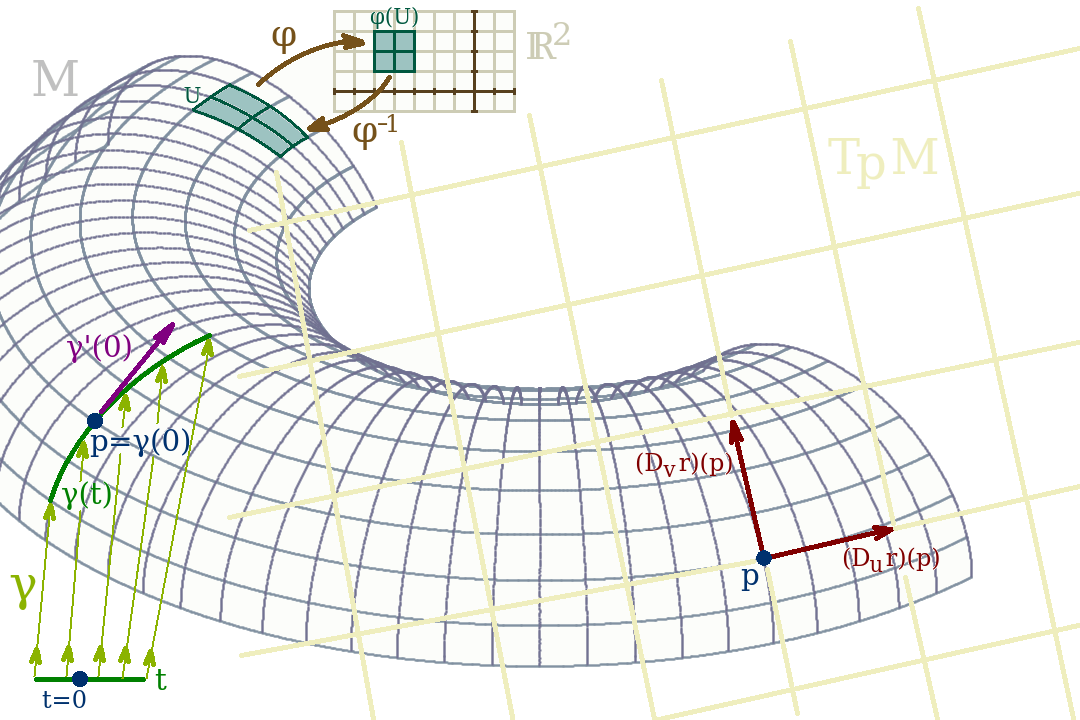
\includegraphics[width=140mm]{img/Torus.png}
\caption{Torus}
\label{img:Torus}
\end{figure}

\end{document}



